\documentclass["../Cours.tex"]{subfiles}

\begin{document}

\chapitre{Droites parallèles et perpendiculaires}

\partie{Définitions}
\definition{Deux droites sont sécantes si elles ont un point d'intersection.}

\illustration{
    \begin{center}
        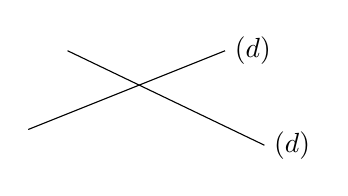
\begin{tikzpicture}
            \draw (0,0) -- (2.5,1) node[right]{$(d)$};
            \draw (0.5,1) -- (3,-0.2) node[right]{$(d)$};
        \end{tikzpicture}
    \end{center}    
}

\definition{Deux droites sont perpendiculaires si elles sont sécantes et elles forment un angle droit.}

\illustration{
    \begin{center}
        \begin{tikzpicture}
            \draw (0,0) -- (2,0) node[right]{$(d)$};
            \draw (1,-1) -- (1,1) node[above]{$(d')$};
            \fill (1,0) rectangle +(0.2,0.2);
        \end{tikzpicture}
    \end{center}
}

\notation{$(d)$ et $(d')$ sont perpendiculaires s'écrit << $(d) \perp (d')$ >>.}

\definition{Deux droites sont parallèles si elles ne sont pas sécantes.}

\illustration{
    \begin{center}
        \begin{tikzpicture}
            \draw (0,0) -- (2,0) node[right]{$(d')$};
            \draw (0,1) -- (2,1) node[right]{$(d)$};
        \end{tikzpicture}
    \end{center}
}

\notation{$(d)$ et $(d')$ sont parallèles s'écrit << $(d) \paral (d')$ >>.}

\clearpage
\EXERCICES
\begin{questions}
    \exercice Sur chaque dessin, trace : en vert, la droite $(d_1)$ \textbf{perpendiculaire} à la droite $(d)$ passant par $A$, puis en rouge, la droite $(d_2)$ \textbf{parallèle} à la droite $(d)$ passant par $B$.

    \begin{center}
        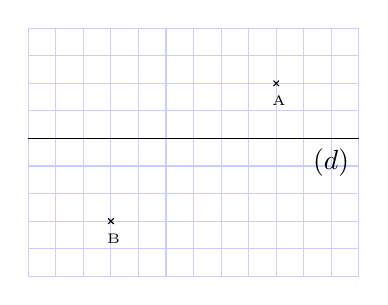
\begin{tikzpicture}[scale=0.35]
            \draw[thin,blue!20!white] (0,0) grid (12,9);
            \draw (0,5) -- (12,5) node[below left]{$(d)$};
            \draw (9,7) ++(0.1,0.1) -- ++(-0.2,-0.2) ++(0,0.2) -- ++(0.2,-0.2) node[below]{\tiny{A}};
            \draw (3,2) ++(0.1,0.1) -- ++(-0.2,-0.2) ++(0,0.2) -- ++(0.2,-0.2) node[below]{\tiny{B}};
        \end{tikzpicture}\hspace{0.1\linewidth}
        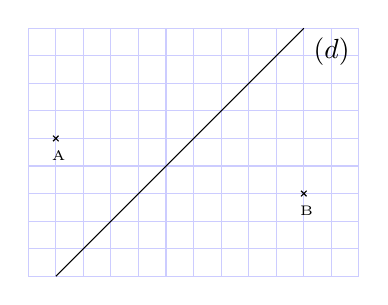
\begin{tikzpicture}[scale=0.35]
            \draw[thin,blue!20!white] (0,0) grid (12,9);
            \draw (1,0) -- (10,9) node[below right]{$(d)$};
            \draw (1,5) ++(0.1,0.1) -- ++(-0.2,-0.2) ++(0,0.2) -- ++(0.2,-0.2) node[below]{\tiny{A}};
            \draw (10,3) ++(0.1,0.1) -- ++(-0.2,-0.2) ++(0,0.2) -- ++(0.2,-0.2) node[below]{\tiny{B}};
        \end{tikzpicture}\hspace{0.1\linewidth}
        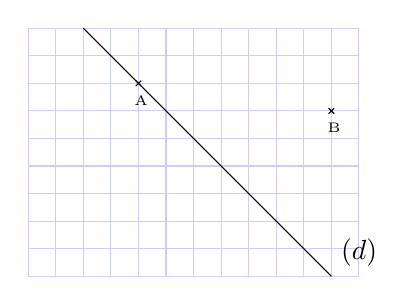
\begin{tikzpicture}[scale=0.35]
            \draw[thin,blue!20!white] (0,0) grid (12,9);
            \draw (2,9) -- (11,0) node[above right]{$(d)$};
            \draw (4,7) ++(0.1,0.1) -- ++(-0.2,-0.2) ++(0,0.2) -- ++(0.2,-0.2) node[below]{\tiny{A}};
            \draw (11,6) ++(0.1,0.1) -- ++(-0.2,-0.2) ++(0,0.2) -- ++(0.2,-0.2) node[below]{\tiny{B}};
        \end{tikzpicture}
    \end{center}

    \exercice Dans chaque cas, construire la droite $(d_1)$ \textbf{perpendiculaire} à la droite $(d)$ et passant par le point $M$, puis la droite $(d_2)$ \textbf{parallèle} à la droite $(d)$ et passant par le point $N$.

    \begin{center}
        \begin{tikzpicture}[scale=0.5]
            \draw (0,0) rectangle (12,8);
            \draw (2,2) -- (9,7) node[right]{$(d)$};
            \draw (5,2) ++(0.1,0.1) -- ++(-0.2,-0.2) ++(0,0.2) -- ++(0.2,-0.2) node[below]{\tiny{M}};
            \draw (10,4) ++(0.1,0.1) -- ++(-0.2,-0.2) ++(0,0.2) -- ++(0.2,-0.2) node[below]{\tiny{N}};
        \end{tikzpicture}\hspace{0.2\linewidth}
        \begin{tikzpicture}[scale=0.5]
            \draw (0,0) rectangle (12,8);
            \draw (1,6) -- (10,1) node[above]{$(d)$};
            \draw ($(1,6)!0.3!(10,1)$) ++(0.1,0.1) -- ++(-0.2,-0.2) ++(0,0.2) -- ++(0.2,-0.2) node[below]{\tiny{M}};
            \draw (9,6) ++(0.1,0.1) -- ++(-0.2,-0.2) ++(0,0.2) -- ++(0.2,-0.2) node[below]{\tiny{N}};
        \end{tikzpicture}
    \end{center}

    \exercice $A$, $B$ et $C$ sont trois points non alignés.
    \question Tracer la droite $(d_1)$ perpendiculaire à $(AB)$ et passant par $C$.
    \question Tracer la droite $(d_2)$ perpendiculaire à $(BC)$ et passant par $A$.
    \question Tracer la droite $(d_3)$ perpendiculaire à $(AC)$ et passant par $B$.
    \question Comment sont les droites $(d_1)$, $(d_2)$ et $(d_3)$ ?

    \begin{center}
        \begin{tikzpicture}
            \coordinate (A) at (0,0);
            \coordinate (B) at (5,0);
            \coordinate (C) at (3,4);
            \draw ($(A)!-0.1!(B)$) -- ($(A)!1.1!(B)$);
            \draw ($(C)!-0.1!(B)$) -- ($(C)!1.1!(B)$);
            \draw ($(A)!-0.1!(C)$) -- ($(A)!1.1!(C)$);
            \node[below] at (A) {$A$};
            \node[left] at (C) {$C$};
            \node[below left] at (B) {$B$};
        \end{tikzpicture}
    \end{center}

    \exercice $A$, $B$, $C$ et $D$ sont quatre points non alignés.
    \question Placer les points $R$, $S$, et $T$, milieux respectifs des segments $[AB]$, $[BC]$ et $[CD]$.
    \question Tracer les droites $(RS)$ et $(ST)$.
    \question Tracer la droite $(d_1)$ parallèle à $(RS)$ et passant par le point $T$.
    \question Tracer la droite $(d_2)$ parallèle à $(ST)$ et passant par le point $R$.
    \question Où se coupent les droites $(d_1)$ et $(d_2)$ ?

    \begin{center}
        \begin{tikzpicture}
            \draw (0,0) node[below]{$A$} -- (1,4) node[above]{$B$} -- (4,4) node[above]{$C$} -- (6,1) node[below]{$D$} -- cycle;
        \end{tikzpicture}
    \end{center}

    \exercice Sur une feuille, effectuer la construction suivante. 
    \begin{itemize}
        \item Tracer un carré de côté \qty{16}{\centi\metre}.
        \item Placer les points $A$, $B$, $C$ et $D$ au milieu de chacun de ses côtés.
        \item Tracer les diagonales et les segments $[AC]$ et $[BD]$.
        \item À partir du point $A$, construire une ligne de perpendiculaires comme sur la figure ci-après. 
        \item Recommencer ensuite à partir des points $B$, $C$ et $D$.
    \end{itemize}

    \begin{center}
        \begin{tikzpicture}[scale=2]
            \draw (-2,-2) rectangle (2,2);
            \draw (-2,-2) -- (2,2) (2,-2) -- (-2,2) (-2,0) node[left]{$D$} -- (2,0) node[right]{$B$} (0,-2) node[below]{$C$} -- (0,2) node[above]{$A$};
            \foreach \angle in {0,90,180,270} {
                \foreach \i in {0,...,3} {
                    \tikzmath{ \r=2/pow(2,\i); \f=0.03; }
                    \draw[rotate=\angle+90*\i] (0,\r) -- ++({-\r/2}, {-\r/2}) -- ++(0,{-\r/2});
                    \fill[rotate=\angle+90*\i] ({-\r/2},{\r/2}) -- ++(\f,\f) -- ++(\f,-\f) -- ++(-\f,-\f) -- ++(-\f,\f);
                    \fill[rotate=\angle+90*\i] ({-\r/2},0) rectangle ++({sqrt(2)*\f},{sqrt(2)*\f});
                };
            };
        \end{tikzpicture}
        \begin{tikzpicture}[scale=2]
            \draw (-2,-2) rectangle (2,2);
            \fill (2,0) -- (2,2) -- (0,2) -- (-1,1) -- (-1,0) -- (-0.5,-0.5) -- (0,-0.5) -- (0.25,-0.25) -- 
        \end{tikzpicture}
    \end{center}
\end{questions}

\end{document}